\documentclass[11pt]{article}

% -- Semantics stuff
%     I defined a couple of special commands (see examples in the text below) to make
%     writing inference rules and judgements easier.
\newcommand{\br}[1]{\langle #1 \rangle}
\def\Yields{\Downarrow}

% -- Page size
\textheight     9.0truein
\textwidth      6.5truein
\topmargin     -0.5truein
\oddsidemargin  +0.0truein
\evensidemargin +0.0truein
\usepackage{amssymb}
\usepackage{amsmath}
\usepackage{fullpage}
\usepackage{enumerate}
\usepackage[mathscr]{euscript}
\usepackage{graphicx}
\usepackage{algorithm}
\usepackage{algpseudocode}
\renewcommand{\theenumi}{\roman{enumi}}

\newtheorem{theorem}{Theorem}[section]
\newtheorem{lemma}[theorem]{Lemma}
\newtheorem{proposition}[theorem]{Proposition}
\newtheorem{corollary}[theorem]{Corollary}

\newenvironment{proof}[1][Proof]{\begin{trivlist}
\item[\hskip \labelsep {\bfseries #1}]}{\end{trivlist}}
\newenvironment{definition}[1][Definition]{\begin{trivlist}
\item[\hskip \labelsep {\bfseries #1}]}{\end{trivlist}}
\newenvironment{example}[1][Example]{\begin{trivlist}
\item[\hskip \labelsep {\bfseries #1}]}{\end{trivlist}}
\newenvironment{remark}[1][Remark]{\begin{trivlist}
\item[\hskip \labelsep {\bfseries #1}]}{\end{trivlist}}

\newcommand{\qed}{\nobreak \ifvmode \relax \else
      \ifdim\lastskip<1.5em \hskip-\lastskip
      \hskip1.5em plus0em minus0.5em \fi \nobreak
      \vrule height0.75em width0.5em depth0.25em\fi}


% -- Document title (appears at top)
\title{Bayesian Modeling in Untargeted Metabolomics}
\author{Alex Tong}
\begin{document}
\maketitle

\section{Background}

I've been working on this project starting in February 2016 with Soha Hassoun. My contribution has been in the probabilistic model design and test. In the spring, we started with a Bayesian Network designed in BayesNet ToolBox a Matlab package \cite{bayesnet}. We found that the tool was not quite right for our needs, so we moved to $PyMC$, a python package built around sampling Bayesian Networks using various MCMC sampling techniques. All code for this project can be found here: https://github.com/atong01/metabolomics-generative-model

\section{Introduction}

Metabolomics uses analyzes complex biological samples by attempting to measure metabolomic compounds. Liquid chromotography mass spectrometry (LC/MS) is able to detect thousands of metabolites in a sample \cite{LCMS}. An interesting question is one of pathway activity. Given we know many of the cell pathways of our sample, we can be informed about how our observations might affect our prior beliefs on the activity of those pathways. We propose a Bayesian interpretation of pathway activity given observations in the mass spectrometry feature space. Given a mass spectrometry measurement on a biological sample of known origin, the posterior distribution on pathway activity is affected by the given sample. We form a generative model of pathway-metabolite production. By informing our prior distribution over pathway activity with new measurements we hope to also propose a set of candidate pathways for further analysis with more accurate targeted metabolomics.

We present 4 models. We use Bayesnet in Matlab, $PyMC$, $PyMC3$, and $PyStan$ to implement these models.

\section{Method}
\subsection{Overview}

Previously, candidate compounds were estimated with statistical tools such as $MetFrag$ on LC/MS fragmentation peaks. We add a post-processing step to compound database lookup and statistical fragment reconstruction techniques to add in known biological context on the sample to improve candidate metabolite predictions. This workflow is show in Figure \ref{workflow}. We use the addition of the $KEGG$ database for pathway metabolite membership as a formulation for our probabilistic model. 

\begin{figure}
\centering
\includegraphics[width=10cm]{Workflow}
\caption{Shows workflow of project}
\label{workflow}
\end{figure}

\subsection{Intuition}

Next we present some intuition on how pathway activity affects compound presence. Many metabolites are present in many pathways. This means that one metabolite could have come from one or many of those pathways. A compound that is a member of many pathways is less informative than one that is a member of a single pathway. A pathway should generate all of its metabolites, but many metabolites do not get picked up by the measurement tool. Therefore, even if a compound does not show up as observed, there is still a high chance that the pathway that produces that compound could be active. Lastly, there are some pathways that are more likely to be active than others. Pathways that are essential to cell function are much more likely to be active based on the prior than those we know are only active in a disease state for example. 

\subsection{Dataset}
We first combine 3 datasets using different settings on the mass spectrometry device, \\
$\{HilNeg, HilPos, SynNeg\}$. We used $MetLin$ and $HMDB$ databases to match spectrometry data sources with known compounds. We used the $MetFrag$ tool to find potential matches to compounds with unknown signatures through fragmentation data. Figure \ref{fig:venn1} shows the set of compounds detected by $Metfrag$ in green, those detected by $Metlin$ or $HMDB$ in red and those in the model in blue. A large proportion of the observed data is of compounds not captured in the pathway data. This is not a surprise as all of these datasets are extremely general and contain compounds that are not related to our sample. In this dataset we have 86 pathways and 1533 compounds. This means that we will be forced to use approximate inference methods such as Gibbs sampling on our bayesian network as exact inference will be computationally infeasible. 

\begin{figure}[h]
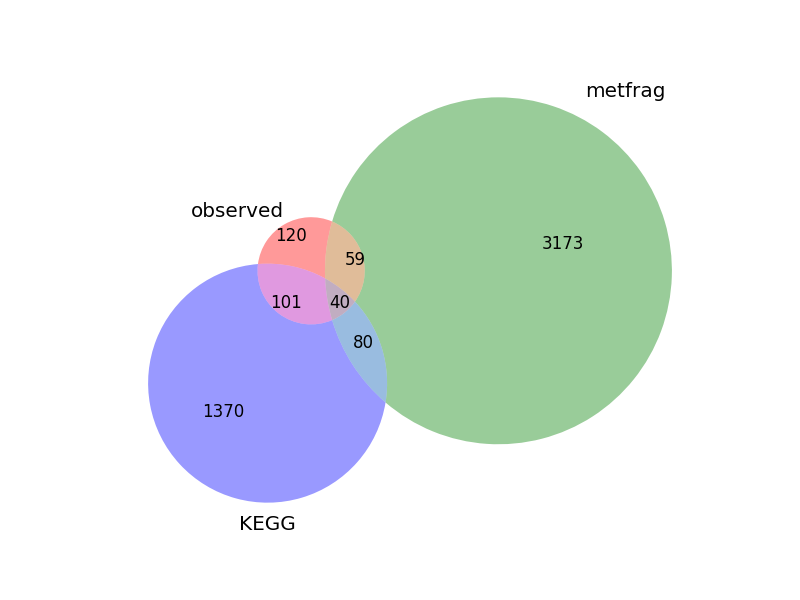
\includegraphics[scale=0.5]{Venn_all_basic}
\centering
\caption{Venn Diagram of Dataset sizes}
\label{fig:venn1}
\end{figure}
\subsection{Approach 1: Generative Model with Virtual Evidence}

\subsubsection{Overview}

Our first approach was a custom generative model. This approach gives a model that hopes to balance the task of capturing the most significant predictive features with the benefits of a simple and computationally efficient model. We attempt to encode our biological knowledge of known pathways by first sampling pathway activity levels and subsequently sampling related metabolite activity levels for each pathway. We then use a concept known as Virtual Evidence to encode our uncertainty in our observation data \cite{Bilmes04onvirtual}.

\subsubsection{Virtual Evidence}

Virtual evidence is a generalization of evidence on Bayesian networks \cite{Bilmes04onvirtual}. Typical Bayesian evidence comes in the form of an observed assignment to a subset $O$ of the network's nodes. All nodes in $O$ have hard assignments, i.e. their state is known with probability equal to 1. Virtual evidence allows evidence on nodes to come in as a probability distribution on possible states. Suppose we have four imperfect measurement sources, which we trust equally. Then suppose that three of these report the coin is heads and the fourth reports the coin is tails. In this case, we could use majority vote to report the coin as heads, or we might want to say we observe a binary node $X$ as 1 with probability $.75$. This keeps the uncertainty of our measurement within the model, and is a strict generalization of evidence as we could put a distribution on $X$ with $P(heads) = 1$. 

The question then is how do we implement Virtual Evidence in a Bayesian network? We do so by creating a Virtual child node to each evidence node, and encoding the evidence probability distribution within the conditional probability table associated with the transition from the evidence node $e_i$ to our virtual node $v_i$. We then provide observation $v_i = 1$ to complete our virtual evidence on node $e_i$. 

\begin{table}[]
\centering
\caption{Conditional Probability Table between evidence node $E$ and associated virtual node $V$}
\label{cpt}
\begin{tabular}{lll}
E & V & P(V | M) \\
0 & 1 & 0.25     \\
1 & 1 & 0.75    
\end{tabular}
\end{table}

Table \ref{cpt} shows a portion of the conditional probability table of $P(v_i | e_i)$. Notice that there are no values for $v_i = 0$. This is because we always observe node $v_i = 1$, and therefore the probability $P(v_i = 0 | e_i)$ is irrelevant. 

\subsubsection{Model 1 Specification}
Parameters:
\begin{itemize}
\item[$\lambda_p$:] Probability that a pathway is active
\item[$\mu_0$:] Probability that a feature is present given inactive pathway
\item[$\mu_1$:] Probability that a feature is present given active pathway
\end{itemize}

Variables:
\begin{itemize}
\item [$a_p$:] IRV indicating pathway $p$ activity
\item [$b_{p,f}$:] IRV indicating feature f is associated with pathway p
\item[$o_{p,f}$:] IRV indicating whether feature $f$ associated with pathway $p$ is present in the sample due to pathway $p$
\item[$m_f$:] IRV indicating whether feature $f$ is present in the sample
\item[$v_f$:] IRV (virtual evidence on feature f
\end{itemize}

Generative Model Prior:
\begin{itemize}
\item [$P_p$:] $Bernoulli(\lambda_p)$ for $p = 1 ... P$
\item [$o_{p,f} | P_p, \mu$:] $Bernoulli(\mu_{P_p})$ for $f$ in Features($p$)
\item [$M_f$]  $= (1 -  \prod_p (1 - o_{p,f}))$ Equivalent to logical OR
\item [$v_f$] $= Bernoulli$(Measured P($f$))
\end{itemize}

Observation:
\begin{itemize}
\item [$v_f$] $ = 1$
\end{itemize}

\begin{figure}
\centering
\includegraphics[width=10cm]{v1}
\caption{Shows the Plate notation for our Bayesian network model}
\end{figure}

Posterior:

\begin{align}
p(o | \lambda, \mu_0, \mu_1, b_{p,f}, a_p) &= \prod_p \prod_{f} (\mu_{a_p}^{o_{p,f}} (1-\mu_{a_p})^{(1-o_{p,f})})^{b_{p,f}} \\
p(m | o, b) &= \prod_f m_f = \prod_f (1 - \prod_p (1 - o_{p,f})^{b_{p,f}}) \\
p(\lambda, \mu_0, \mu_1, a, o, m) &= p(a | \lambda )p(\lambda) p(\mu_0) p(\mu_1) p( o | \lambda, \mu_0, \mu_1, b_{p,f}) p(m | o) \\
p(\lambda, \mu_0, \mu_1, a, o, m | v = \mathbf{1}) &= \frac{p(v | \lambda, \mu_0, \mu_1, a, o, y) * p(\lambda, \mu_0, \mu_1, a, o, m)}{p(v = \mathbf{1})}  \\
&\propto p(v | m) * p(\lambda, \mu_0, \mu_1, a, o, m) 
\end{align}
%p(\alpha | v = \mathbf{1}) &= 

Description:
Equation 1 shows the likelihood of a given set of $o$ variables. For example, if I wanted to calculate the probability of all $o_{p,f}$ variables being zero, I would need all given hyper-parameters, $\lambda, \mu_0, \mu_1$, and the values of $a_p$. The likelihood as stated is a function of $p$ variables, $a_{1...p}$. Note that with this likelihood function, it is simple to calculate the likelihood $P(o | \lambda, \mu_0, \mu_1, a)$, In fact, for a given $o_{p,f}$, we can calculate $p(o_{p,f} | a_p, b_{p,f}) = \mu_{a_p}^{o_{p,f}} (1-\mu_{a_p})^{(1-o_{p,f})}$ or 
$$p(o_{p,f} = 1 | a_p, b_{p,f}) = \mu_{a_p}$$
$$p(o_{p,f} = 0 | a_p, b_{p,f}) = 1-\mu_{a_p}$$
Equation 2 shows the likelihood of a set of metabolite observations given $o$. for example, the probability of getting $m_1 = 1, m_2 = 0, m_3 = 1$ given all of $o$, is a constant.\\\\
Equation 3 shows the likelihood over all hidden variables. This is derived from looking at our bayesian network, as each variable is independent.\\\\
Equation 4 shows the model likelihood given our observation of our virtual nodes. This is derived from bayes rule. \\\\

$$p(v_f | m_f) = P(metfrag)  * P(\pi)$$

Reasonable Values:
\begin{itemize}
\item $\pi$ should be nominally quite low, and may be lower for some metabolites than others possibly with the idea that larger molecules are harder to detect as there are more possible fragments.
\item We will start with $\mu_0 = 0.001$ and $\mu_1 = 0.999$ as values very close to 0 and 1. 
\item We will start with $\lambda = 0.5$, but would like to move to a model where we can incorporate more reasonable priors separately on each pathway, something like a $\lambda_p$ for $p = 1...P$. 

\end{itemize}



\subsubsection{Posterior Distribution Calculation}

We use this model to calculate a posterior distribution over pathway activities $a_p$. We attempted Gibbs sampling using $PyMC$, as full inference on a network of this size is computationally infeasible. We ran the sampler for $10000$ iterations, burning the first $1000$ samples, and keeping every $10$th sample. These parameters are assumed to provide ~$900$ independent samples on our posterior distribution on pathway activity. 

\subsubsection{Findings}

We implemented this model first in Matlab and then re-implemented it in $PyMC$. We found the Matlab version sampled from the distribution too slowly. Once we re-implemented in $PyMC$, we found that the model was too restrictive to converge. This model relies on a lot of binary variables. A pathway is either active or it is not. A metabolite is either present in the sample or it is not. These assumptions make sense in the physical context. It is true that a metabolite is either present or not present. This correspondence means that it is extremely easy to relate the posterior distribution calculated on the hidden variables in this model to the real world. However, with these binary assumptions we get into trouble while sampling. Take for example sampling the distribution on $n$ coins. Suppose in the true distribution, the probability of all heads is $\frac{1}{2}$, and all other states are equally probable occurring with probability $\frac{1}{2 * (2 ^ n - 1)}$. If we sample from the true distribution it will quickly become clear that about $\frac{1}{2}$ of the samples are all heads, however with Gibbs sampling we will switch between sampling approximately $2 ^ {n - 1}$ vectors of all heads and $2 ^ {n-1}$ non all heads vectors. 

We reach a failure mode when we sample a pathway with many unlikely metabolite members. This will mean that in the next sample, that pathway probability will be lower. This will in turn lower the probability of seeing any of the metabolites in that pathway. This leads to a cycle of decreasing probability where we ignore the observed values and find a relatively likely posterior distribution of all deactivated pathways and no observed metabolites. A potential solution to this problem is blocked sampling, where variables are grouped into blocks which are sampled together. By sampling values for all pathways together, and all metabolites together than we will be less likely to get stuck in such a spiral of decreasing probabilities. We did not attempt blocked gibbs sampling as it would require a sampler customized for our problem space. 

\subsection{Approach 2: Generative Model with Continuous Variables}

In order to minimize the failure mode found in the first approach, we try a second approach using continuous activation variables. Conceptually, this means that instead of picturing a pathway as active or inactive with an associated probability, we have an activation level for each pathway with activation level $a \ge 0$. This means that we give up some interpretability of the model. We are no longer easily able to assess the activity probability of each pathway in absolute terms, but are still able to look at the relative activity between pathways. Similarly we move to an activation variable on each metabolite. 

\subsubsection{Model 2 Specification}
Model 2 has a couple parts. We use Gamma distributions to condition activation levels of metabolites on activation levels of pathways. The target function is designed to learn a base level of detection for metabolites, that is we need to model the fact that even if a metabolite is present in the sample it could still remain unobserved. We still have the same generative model structure as in the first approach. We sample pathway activations which drive metabolite activations.

This time we consider an object function $target$ which also puts a prior on reasonable values for our model. We design target so that when a metabolite is observed, we increase the model likelihood based on $\beta_m$ with some normalization values, and when a metabolite is not observed then this can be attributed to our detection probability $\epsilon$. This is made such that an observed metabolite has a large effect on our posterior vs an unobserved metabolite which has a very small effect on our posterior. This is reasonable as there is more information contained in a positive example than a negative one as we can attribute a negative observation to the probability of not detecting a metabolite even if it exists in the sample. \\\\
Parameters:
\begin{itemize}
\item[rate\_prior:] Prior pathway activity level
\item[$\epsilon$:] Detection probability level
\item[$a_p$:] Pathway activation levels
\item[$b_{p,m}$:] Pathway metabolite activation levels
\item[$target$:] total model probability
\end{itemize}

Generative Model:
\begin{itemize}
\item [$y_m$] $= 1$ if metabolite m is observed, otherwise $0$.
\item [$a_p \sim$] Gamma(rate\_prior, 1)
\item [$b_{p,m} \sim$] Gamma($a_p$, 1) for each metabolite
\item [$\beta_m \sim$] $\sum_p b_{p,m}$.
\item [$target_m$] $ = \begin{cases}
 log(\epsilon) - \frac{1}{2} * \beta_m + log( 1 - e ^ { - \beta_m}) & \text{ if } y_m= 1 \\ 
 log((1 - \epsilon) + \epsilon * e ^ {-\beta_m}) & \text{ if } y_m = 0
\end{cases}$
\item[$target$] $ = \sum_m \text{target}_m$
\end{itemize}

\subsubsection{Findings}

We implemented this model in $PyStan$. We use PyStan for its No U Turn Sampler (NUTS). This sampler is much more efficient with continuous variables, using gradient based methods instead of random walk to determine the next sample. PyStan is built in such a way that it allocates memory for all samples at the start of the program. This means that a long sampler is memory bound. We ran on the tufts cluster on the largemem partition. The model did not converge when measured by n\_eff and r\_hat measures. This is probably due to the large number of variables that need to be sampled. $b$ is a $P \times M$ matrix, representing over 100,000 variables. This model does converge on small test examples and performs as expected. This implies that with enough samples the model is likely to converge, the question then becomes how many samples are necessary. In the next model we attempt to lower the number of latent variables in the model which we hope will converge more quickly.

\subsubsection{Further Steps}

Further work on this model could be in determining on what scale it is effective and why. We know that it is effective on the order of 3 pathways and 3 metabolites, but is ineffective on 86 pathways and 1533 metabolites. There is a large gap between these two test cases, and a more accurate figure could help guess how many samples are necessary and what size is feasible to solve by NUTS sampling. We also attempted on 10, 20, and 30 pathways with the full 1533 metabolites but these also failed to converge.

\subsection{Approach 3: Generative Model: $O(M+P)$ Latent Variables}

We now present a model where we have a single activation level for each pathway and a single activation level for each metabolite. This greatly decreases the number of variables that need to be sampled. This model is similar to the Poisson Factorization model described in the paper ``Scalable Recommendations with Poisson Factorization" \cite{Poisson13}. The difference comes in the observations, we have continuous outputs where they work with discrete ratings, for example 1-5 stars. 

\subsubsection{Model 3 Specifications}

Parameters:
\begin{itemize}
\item[met\_mask:] Metabolite Mask $ P \times M$ dimension matrix with 1 in slot $p,m$ if metabolite $m$ is a member of pathway $p$.
\item[$k_p \sim$] Gamma(activity\_shape, activity\_rate)
\item[$\theta_m \sim$] Gamma(met\_mask * detection\_shape, detection\_rate)
\item[$y_m \sim$] Gamma(met\_mask * k, $\frac{1}{\theta}$)
\end{itemize}

\subsubsection{Findings}

We implemented this model in $PyStan$. We ran it with a number of different shape and rate parameters. The model again converges on small test examples but as measured by n\_eff and r\_hat parameters, it fails to converge on the full dataset.

\subsubsection{Future Work}

The Poisson Factorization model by Gopalan et al. should be directly applied to this problem \cite{Poisson13}. The downside of this model would be that there is no way to incorporate the metabolite mask into the sampling. Incorporating the mask would require diving into the Poisson Factorization code published here: https://github.com/premgopalan/hgaprec

\subsection {Poisson Model 4}
Definitions
\begin{itemize}
    \item $p_m$: probability of observation on metabolite m, $p_m \in [0,1]$
\end{itemize}
Parameters
\begin{itemize}
    \item $a_p \sim Gamma(*,*)$
    \item $\epsilon = 1.0\times10^{-4}$
    \item $b_{p,m} \sim Gamma(a_p, 1)$
    \item $\beta_m \leftarrow \sum_p b_{p,m}$
    \item $\gamma_m \sim Bernoulli(1 - e^{-\beta_m})$
\end{itemize}
Original Potential Function\\
$f(m,\epsilon) = \begin{cases}
 p_m * (1-e^{-\beta_m}) & \text{ if } m \in Evidence \\ 
 \epsilon * e ^ {-\beta_m}& \text{ else}
\end{cases}$
\\\\
Modified Potential Function \\
$y(m) = 1 - e^{-\beta_m} \\
\alpha = \frac{1}{1 - p_m}\\
g(m,\epsilon) = \begin{cases}
 y(m) & \text{ if } m \in Evidence \\ 
 (1 - y(m)) * y(m) ^ {\alpha - 1} &\text{ elif } m \in SoftEvidence\\
 \epsilon * e ^ {-\beta_m}& \text{ else}
\end{cases}$\\
The soft evidence portion of $g(m, \epsilon)$ is proportional to a beta distribution pdf on $y(m)$ with $\alpha = \frac{1}{1 - p_m}, \beta = 2$. These parameter settings are based on the fact that we would like $g(m, \epsilon)$ to be maximal at $p_m$. \\
$$\begin{align*}
p_m &= \frac{\alpha - 1}{\alpha + \beta - 2} \\ 
\beta &= 2 \\ 
p_m &= \frac{\alpha - 1}{\alpha} \\
\alpha &=  \frac{1}{1 - p_m}
\end{align*}$$

\subsubsection{Questions}
\begin{itemize}
    \item Would it be beneficial to normalize $g(m, \epsilon) \text{ where } m \in SoftEvidence$? \\
    $B(\alpha, \beta) = \frac{\Gamma(\alpha) \Gamma(\beta)}{\Gamma(\alpha + \beta)} \\
    g(m,\epsilon) = \begin{cases}
 y(m) & \text{ if } m \in Evidence \\ 
 \frac{(1 - y) * y ^ {\alpha - 1}}{B(\alpha, \beta)} &\text{ elif } m \in SoftEvidence\\
 \epsilon * e ^ {-\beta_m}& \text{ else}
\end{cases}$\\
\end{itemize}
This question remains untested.

\subsubsection{Findings}

This model was implemented in $PyMC$. When run for 300,000 samples this model still exhibits instability. This implies that we need to run for more iterations until convergence. This makes sense as there are many local minima in this model. $PyMC$ uses a random walk type sampler. This means that convergence on continuous variables may take a long time as samples are uneducated guesses. Future Implementation in $PyMC3$ may be a useful exercise. 

\section{Implementation Details}

All of the code can be found in the git repository which is divided into three main sections titled ``Matlab", ``pymc", and ``pystan". 

\subsection{Matlab}
matlab/modelF/modelF.m is the file containing the last relevant Matlab model. We used likelihood weighted inference engine. This is an exact inference method and does not scale well with data size. We use the noisy\_or conditional probability table (CPT) type for edges from pathways to metabolites. This allows us to model the fact that a metabolite should be active if any of its pathways is active. 

We then establish probability tables to the virtual nodes using the probability of evidence in the table during graph construction. We are then able to set as evidence all virtual nodes with the value 1. 

\subsection{$PyMC$}

There are two versions of $PyMC$. Standard $PyMC$ and $PyMC3$. $PyMC$ has better documentation at this time, but $PyMC3$ has some features that were built after the final support of $PyMC$. The NUTS function (No U-Turn Sampler) in $PyMC3$ makes $PyMC3$ particularly attractive. We implemented most functions in $PyMC$ standard first as there is better documentation. There are two main branches of the $PyMC$ code. The latest version of model 1 can be found in pymc/vx, and the latest version of model 4 can be found in pymc/poisson3.

\subsection{$PyStan$}

All $PyStan$ code can be found in the stan directory. There are many batch scripts with associated output in slurm format. These are useful to keep organized on how each test output was obtained. Batch scripts can be run again for repeatable results. 

\section{Conclusion}

In conclusion, our method seems promising, however there are many unanswered questions. The first of which is how to incorporate more biological information with the assumption that as our model becomes more biologically accurate, our model accuracy will increase. We currently treat pathways as bags of compounds. If a pathway is active then all of its members should be present. This is however far from reality. Pathways can be expressed much more accurately as graphs of with nodes of compounds with directed or undirected reactions between them. Furthermore, a single pathway can have many active and inactive portions. Using the graph structure of pathways can lead to conclusions on with metabolites might be more informative than others for the same pathway. We might want to try some measure of centrality of a metabolite with the idea that a more central metabolite might have more importance. There are many other possible sources of information that could be encoded into the model. Hopefully with a larger dataset we may be able to learn some of these parameters. 

We have had trouble getting our models to converge while sampling. The sparsity of our data should be better modelled with existing methods for sparse matrix factorization such as recommender systems. 

\section{Acknowledgments}

Thanks to Nicholas Alden, Vlad Porokhin, Neda Hassanpour, Kyongbum Lee, Soha Hassoun who are also working on this project. As well as thanks to Jan-Willem Van de Meent, professor at Northeastern University.

\section{CodeBase}

All code and results associated with this project can be found at: \\https://github.com/atong01/metabolomics-generative-model

\bibliographystyle{unsrt}%Used BibTeX style is unsrt
\bibliography{sample}

\end{document}
